\section{Optimal torque control}


\begin{frame}{Optimal torque control}{System constraint}
    \begin{columns}
    \begin{column}{0.4\framewidth}
        \only<2>{\colorbox{lightblue}{ Objective: \textcolor{red}{Minimize Joule losses} }}
         \begin{eqnarray*}
            \only<3-4>{&\underset{i_d,i_q}{\textbf{min}} \quad i_{dq}^\top i_{dq},\quad \textbf{such that}\\}
            &\tikz[remember picture,baseline=(idqeq.base)]{\node[inner sep=0pt](idqeq){$i_{dq}^\top i_{dq} - i_{max}^2 \leqslant 0$};}\\
            %\only<1-2>{&  \tikz[remember picture,baseline=(vdqeq.base)]{\node[inner sep=0pt](vdqeq){$v_{dq}^\top v_{dq} - v_{max}^2\leqslant 0$,};} \\}
            \only<1-3>{&  \tikz[remember picture,baseline=(vdqeq.base)]{\node[inner sep=0pt,align=center](vdqeq){$\textcolor{orange}{A(\omega)} i_d^2 + \textcolor{orange}{B(\omega)}i_di_q + \textcolor{orange}{C(\omega)}i_q^2+$ \\ $ \textcolor{orange}{D(\omega)}i_d + \textcolor{orange}{E(\omega)}i_q + \textcolor{orange}{F(\omega)} \leqslant 0$};} \\}
            \only<4>{&  \tikz[remember picture,baseline=(vdqeq.base)]{\node[inner sep=0pt,align=center](vdqeq){$\textcolor{black}{A(\omega)} i_d^2 + \textcolor{black}{B(\omega)}i_di_q + \textcolor{black}{C(\omega)}i_q^2+$ \\ $ \textcolor{black}{D(\omega)}i_d + \textcolor{black}{E(\omega)}i_q + \textcolor{black}{F(\omega)} \leqslant 0$};} \\}
            %
            \only<1-3>{& \tikz[remember picture,baseline=(taueq.base)]{\node[inner sep=0pt](taueq){$\tau_{em} - \frac{3}{2}p \big( \phi_f +  (L_d - L_q) i_d \big) i_q= 0.$}; }}
            \only<4>{& \tikz[remember picture,baseline=(taueq.base)]{\node[inner sep=0pt](taueq){$\textcolor{red}{\tau_{em}} - \frac{3}{2}p \big( \phi_f +  (L_d - L_q) i_d \big) i_q= 0.$}; }}
         \end{eqnarray*}
         \tikz[remember picture,overlay] {
            %\only<1>{\draw[dashed,very thick,rounded corners,blue] ([xshift=-0.1cm,yshift=0.2cm]idqeq.north west) rectangle ([xshift=0.1cm,yshift=-0.08cm]idqeq.south east);}
            %\only<2>{\draw[dashed,very thick,rounded corners,red] ([xshift=-0.1cm,yshift=0.1cm]vdqeq.north west) rectangle ([xshift=0.1cm,yshift=-0.08cm]vdqeq.south east);}
            %\only<3>{\draw[dashed,very thick,rounded corners,red] ([xshift=-0.1cm,yshift=0.1cm]vdqeq.north west) rectangle ([xshift=0.1cm,yshift=-0.08cm]vdqeq.south east);}
            \only<4>{\draw[dashed,very thick,rounded corners,red] ([xshift=-0.1cm,yshift=0.1cm]taueq.north west) rectangle ([xshift=0.1cm,yshift=-0.08cm]taueq.south east);}
            % \node[right] at ([xshift=0.2cm]idqeq.east) {\textcolor{blue}{Electrical dynamic}};
            }
    \end{column}
    \begin{column}{0.6\framewidth}
    \centering
     %\only<1>{Current constraint in the $i_{dq}$ frame
    %     \centering
    %     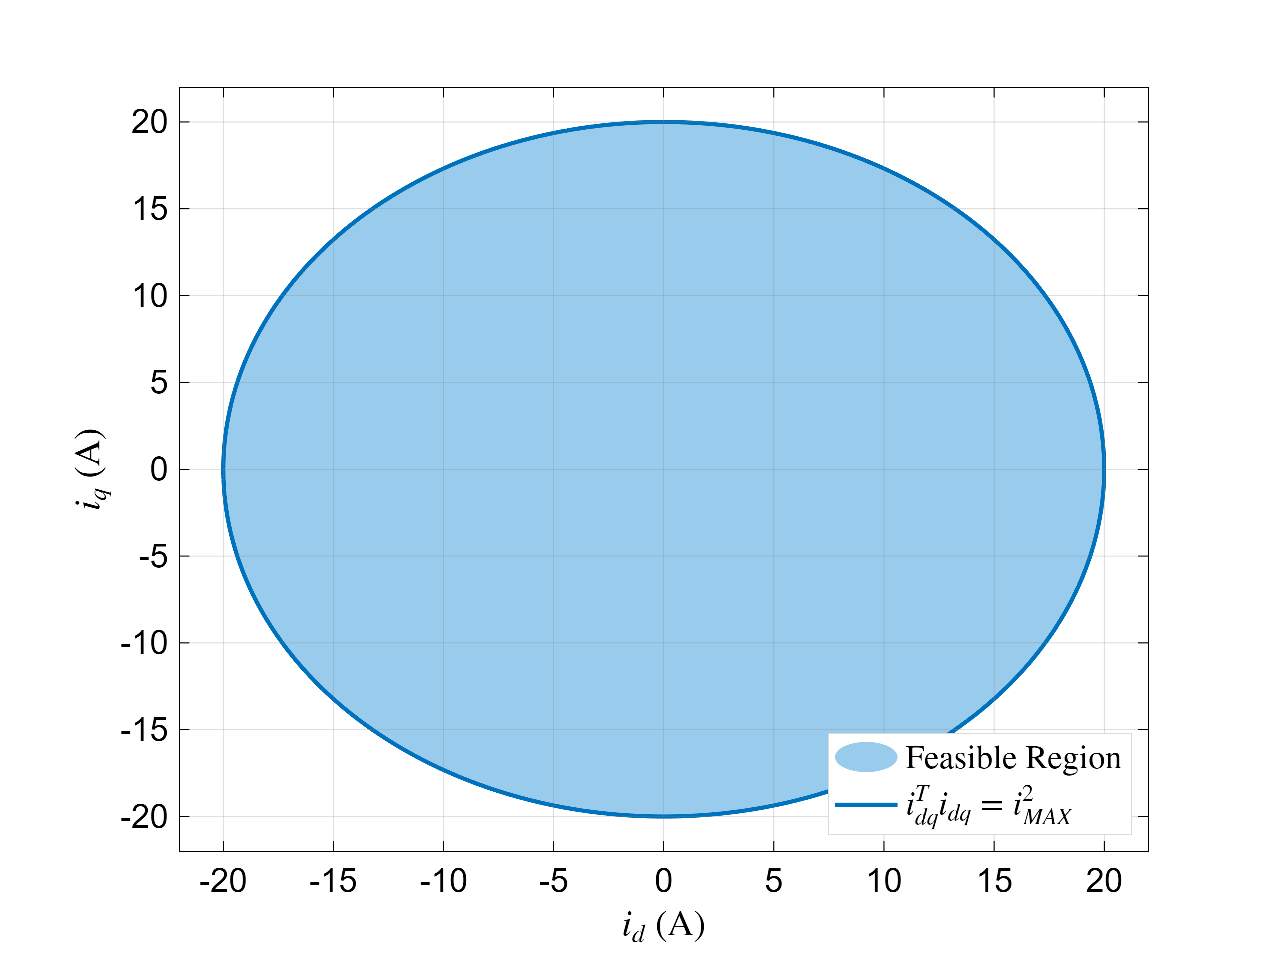
\includegraphics[width=7cm]{pictures/current_constraint_cost.eps}
    %  }
    % %  \only<2>{
    %     Voltage  constraint in the $i_{dq}$ frame
    %      \begin{eqnarray*}
    %         \cancel{L_d \frac{di_d}{dt}} &=& v_d - Ri_d +p L_q\omega i_q = 0, \\
    %         \cancel{L_q\frac{di_q}{dt}} &=& v_q -Ri_q -pL_d\omega i_d -p \phi_f\omega = 0,
    %    \end{eqnarray*}
    %  }
    %  \only<3>{
    %  \begin{center}
    %       \animategraphics[loop,controls,width=1\textwidth]{10}{eps_frames_voltage_animation_filled_with_cost/frame_}{000}{040}
    %   \end{center}
    %  }
     \only<1-2>{
      \begin{center}
         % \animategraphics[loop,controls,width=1\textwidth]{10}{eps_frames_voltage_cost_torque/frame_}{000}{040}
         %%%%%%%%%%%%%%%%%%%%Here Here here 
         \animategraphics[loop,controls,width=1\textwidth]{10}{eps_frames_voltage_animation_torque/frame_}{000}{040}
      \end{center}
     }
     \only<3>{\animategraphics[loop,controls,width=1\textwidth]{10}{eps_frames_voltage_cost_torque_optimal/frame_}{000}{040}
     }
     \only<4> {\animategraphics[loop,controls,width=1\textwidth]{10}{eps_frames_torque_cost_speed_optimal/frame_}{000}{014}
     }
    \end{column}
    \end{columns}
\end{frame}



\subsection{Literature}
\begin{frame}{Optimal torque control}{Literature}
\begin{columns}
    \begin{column}{0.5\framewidth}
    The classical optimal torque control problem:
    \vspace{+0.3cm}
        \begin{eqnarray*}
            &\underset{i_d,i_q}{\textbf{min}} \quad i_{dq}^\top i_{dq},\quad \textbf{such that}\\
            & i_{dq}^\top i_{dq} - i_{max}^2 \leqslant 0\\
            & A(\omega) i_d^2 + B(\omega)i_di_q + C(\omega)i_q^2+ \\
            & \quad D(\omega)i_d + E(\omega)i_q + F(\omega) \leqslant 0\\
            & \tikz[remember picture,baseline=(taueq.base)]{\node[inner sep=0pt](taueq){$ \tau_{em} - \frac{3}{2}p \big( \phi_f +  (L_d - L_q) i_d \big) i_q= 0.$}}
        \end{eqnarray*}
        \tikz[remember picture,overlay] {
        \draw[dashed,very thick,rounded corners,red] ([xshift=-0.1cm,yshift=0.1cm]taueq.north west) rectangle ([xshift=0.1cm,yshift=-0.08cm]taueq.south east);}
    \end{column}
    \begin{column}{0.5\framewidth}
        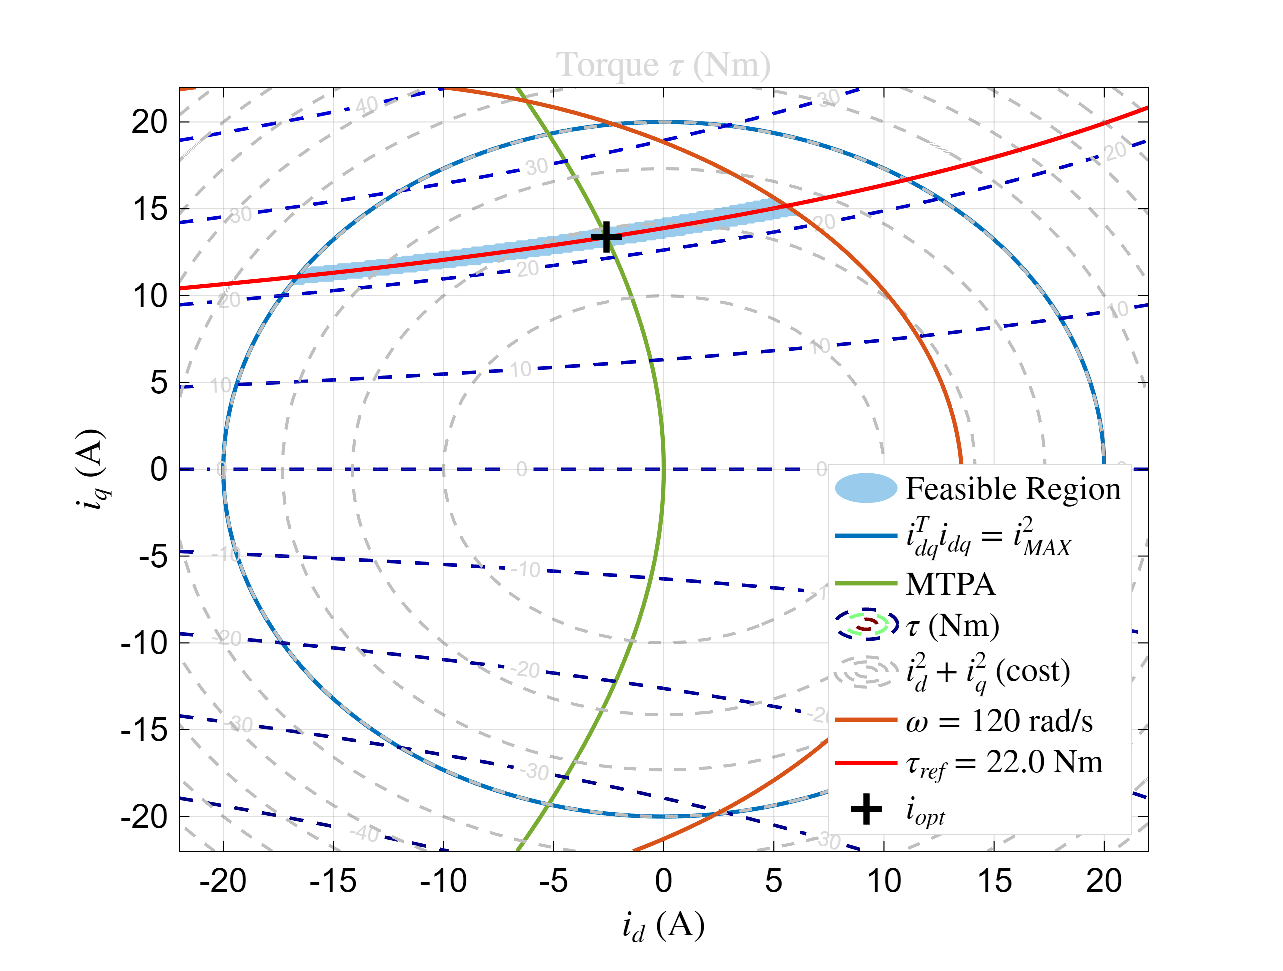
\includegraphics[width=1\columnwidth]{eps_frames_torque_cost_speed_optimal/frame_010}
        %eps_frames_voltage_animation_torque/frame_
    \end{column}
\end{columns}
\textbf{Challenge:} the torque constraint is \textcolor{red}{nonconvex}
\end{frame}

\begin{frame}{Optimal torque control}{Classical approach: Decision tree \footnote{H. Eldeeb et al., "\textbf{A unified theory for optimal feedforward torque control of anisotropic synchronous machines}," \textit{International Journal of Control}, pp. 2273–2302, Oct. 2018.}}
    \begin{columns}[T] % [T] aligns the tops of the columns
        \begin{column}{0.4\textwidth}
            \textbf{Literature approach:} \textcolor{Blue}{\textbf{Decision tree}}

            \vspace{0.4cm}
            \textbf{Operating zones:}
            \begin{itemize}
                \item \textcolor{blue}{MTPC}: No constraint active
                \item \textcolor{orange}{Maximum Current}: Current constraint active
                \item \textcolor{green!60!black}{Field Weakening}: Voltage constraint active
                \item \textcolor{cyan!60!black}{MTPV}: Both constraints active
            \end{itemize}
        \end{column}

        \begin{column}{0.5\textwidth}
            \only<1->{
                \vspace{-1cm}
                    \begin{figure}
                    \centering
                    \includegraphics[width=1.1\columnwidth]{pictures/decision_tree_hq.eps}
                    \caption{Optimal torque control decision tree}
                    \end{figure}
            }
        \end{column}
    \end{columns}
    \only<2>{
     \vspace{0.1cm}
    \begin{center}
    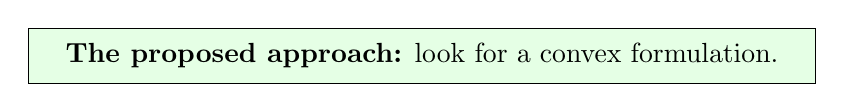
\begin{tikzpicture}
        \node[draw, rectangle, fill=green!10, minimum width=10cm, minimum height=0.7cm] {
            \begin{minipage}{9.5cm}
                \centering
                \textbf{The proposed approach:} look for a convex formulation. 
            \end{minipage}
        };
    \end{tikzpicture}
    \end{center}
    }
\end{frame}


\begin{frame}{Optimal torque problem}{Advantages of the proposed convex formulation \footnote{S. Boyd and L. Vandenberghe, "\textbf{Convex Optimization}," Cambridge University Press, 2004.}}

    \vspace{0.2cm}
    \begin{columns}[t]
        \begin{column}{0.48\framewidth}
            \textbf{The \textcolor{Blue}{convex} formulation}
            \begin{itemize}

                \item \textcolor{Blue}{\textbf{Solvers with polynomial complexity}}
                \item \textcolor{Blue}{\textbf{Scales efficiently}} to complex scenarios
                \item \textcolor{Blue}{\textbf{Easy to add constraints}}
                \item \textcolor{Blue}{\textbf{Guaranteed convergence}} to global optimum
                \item \textcolor{Blue}{\textbf{Easy to integrate}}
                \item \textcolor{Blue}{\textbf{Unified solution}} 
            \end{itemize}
        \end{column}
    %\end{columns}

            \begin{column}{0.48\framewidth}
            \textbf{Decision tree approach:}
            \begin{itemize}
                \item Combinatorial complexity when adding constraints
                \item Difficult to scale up the problem
                 \item Case-by-case analysis for each operating region
            \end{itemize}
        \end{column}
   % \vspace{0.4cm}
    \end{columns}

%     \vspace{0.3cm}
%     \begin{center}
%     \begin{tikzpicture}
%         \node[draw, rectangle, fill=green!10, minimum width=10cm, minimum height=0.7cm] {
%             \begin{minipage}{9.5cm}
%                 \centering
%                 \textbf{Example:} Control $N$ PMSMs on the same power source 
%             \end{minipage}
%         };
%     \end{tikzpicture}
%     \end{center}
 \end{frame}

% \begin{frame}{Optimal torque control}{The proposed approach}
%     \begin{columns}[T] % optional: align top
%         % Left column
%         \begin{column}{0.5\textwidth}
%             \begin{eqnarray*}
%                 &\underset{i_d,i_q}{\textbf{min}} \quad i_d^2+i_q^2,\quad \textbf{such that}\\
%                 & i_{dq}^\top i_{dq} - i_{max}^2 \leqslant 0\\
%                 & A(\omega) i_d^2 + B(\omega)i_di_q + C(\omega)i_q^2+ \\
%                 & \quad D(\omega)i_d + E(\omega)i_q + F(\omega) \leqslant 0\\
%                 & \tikz[remember picture,baseline=(taueq.base)]{\node[inner sep=0pt](taueq){$ \tau - \frac{3}{2}p \big( \phi_f +  (L_d - L_q) i_d \big) i_q= 0.$}}
%             \end{eqnarray*}

%             \begin{center}
%                 \begin{tikzpicture}
%                     \node[draw, rectangle, fill=red!10, minimum width=7cm, minimum height=0.8cm] {
%                         \begin{minipage}{6.5cm}
%                             \centering
%                             \textbf{How to make the problem convex ?}
%                         \end{minipage}
%                     };
%                 \end{tikzpicture}
%             \end{center}

%             \pause
%         \end{column}

%         % Right column
%         \begin{column}{0.5\textwidth}
%             \textbf{The proposed solution:}
%             \begin{center}
%                 \begin{tikzpicture}
%                     \node[draw, rectangle, fill=green!10, minimum width=7cm, minimum height=0.8cm] {
%                         \begin{minipage}{6.5cm}
%                             \centering
%                             \textbf{A change of variable}
%                         \end{minipage}
%                     };
%                 \end{tikzpicture}

%                 \begin{equation*}
%                     i_q = \frac{2}{3p} \frac{\tau}{\phi_f+(L_d-L_q)i_d}.
%                 \end{equation*}
%             \end{center}
%         \end{column}
%     \end{columns}
% \end{frame}

\begin{frame}{Optimal torque control}{The proposed approach}
\begin{columns}[T]

% Left column
\begin{column}{0.5\textwidth}
    \only<1->{
    \textbf{The classical problem:}
\begin{eqnarray*}
&\underset{i_d,i_q}{\textbf{min}} \quad i_{dq}^\top i_{dq},\quad \textbf{such that}\\
& i_{dq}^\top i_{dq} - i_{max}^2 \leqslant 0\\
& A(\omega) i_d^2 + B(\omega)i_di_q + C(\omega)i_q^2+ \\
& \quad D(\omega)i_d + E(\omega)i_q + F(\omega) \leqslant 0\\
& \tikz[remember picture,baseline=(taueq.base)]{\node[inner sep=0pt](taueq){$ \tau_{em} - \frac{3}{2}p \big( \phi_f +  (L_d - L_q) i_d \big) i_q= 0.$}}
\end{eqnarray*}

\begin{center}
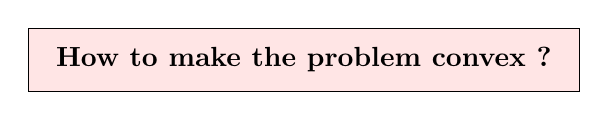
\begin{tikzpicture}
\node[draw,rectangle,fill=red!10,minimum width=7cm,minimum height=0.8cm]{
\begin{minipage}{6.5cm}\centering\textbf{How to make the problem convex ?}\end{minipage}};
\end{tikzpicture}
\end{center}
    }


\end{column}

% Right column
\begin{column}{0.5\textwidth}
    \only<2->{
\textbf{The proposed reformulation:}
\begin{center}
\begin{tikzpicture}
\node[draw,rectangle,fill=green!10,minimum width=7cm,minimum height=0.8cm]{
\begin{minipage}{6.5cm}\begin{center}

\textbf{A change of variable}
\begin{equation*} i_q=\frac{2}{3p}\frac{\tau_{em}}{\phi_f+(L_d-L_q)i_d}. \end{equation*} \end{center}
\end{minipage}};
\end{tikzpicture}
\end{center}
    }
    \only<3->{
The new problem is
\begin{center}
\begin{tikzpicture}
\node[draw,rectangle,fill=green!10,minimum width=7cm,minimum height=0.8cm]{
\begin{minipage}{6.5cm}
    \begin{center}
\begin{eqnarray*}
&\underset{i_d}{\textbf{min}} \quad f(i_d,\tau_{em})\quad \textbf{such that}\\
&c_i(i_d,\tau_{em})\leqslant0\\
&c_v(i_d,\omega,\tau_{em})\leqslant0\\
\end{eqnarray*}
 \end{center}
\end{minipage}};

\end{tikzpicture}
\end{center}
    }

\end{column}
\end{columns}
    \only<4>{\textbf{\textcolor{Blue}{Is the problem convex?}}
    over the set $\mathcal{S} =  \{(i_d, \omega, \tau_{em}) \in \mathbb{R}^3 \:|\: -i_{max} \leqslant i_d \leqslant 0, \: \omega \geqslant 0, \: \tau_{em} \geqslant 0\} $
    }

\end{frame}

\begin{frame}{Optimal torque control problem}{Convexity of the proposed formulation}
\textbf{Question:} Is the reformulated problem convex over $\mathcal{S}$?
\begin{equation*}
\underset{i_d}{\textbf{min}} \quad f(i_d,\tau_{em})\quad \textbf{s.t.}\quad
c_i(i_d,\tau_{em})\leqslant0, \quad c_v(i_d,\omega,\tau_{em})\leqslant0
\end{equation*}

% \only<1>{
% \vspace{0.2cm}
% \begin{block}{Convexity requirements}
% \begin{itemize}
%     \item Objective $f$: \textcolor{blue}{\textbf{convex}} ($f'' \geq 0$)
%     \item Constraints $g_i(x) \leq 0$: \textcolor{blue}{\textbf{convex}} functions
% \end{itemize}
% \end{block}
% }

%\only<2>{
    \vspace{0.3cm}
    \textbf{Analysis over $\mathcal{S}$:}
    \begin{itemize}
        \item[$\checkmark$]  $f(i_d,\tau_{em})$ is \textcolor{blue}{\textbf{convex}}
        \item[$\checkmark$]  $c_i(i_d,\tau_{em})\leqslant 0$ is \textcolor{blue}{\textbf{convex}}
        \item[$\boldsymbol{?}$]  $c_v(i_d,\omega,\tau_{em})\leqslant 0$ is \textcolor{red}{\textbf{convex}} ?
    \end{itemize}
    \vspace{0.3cm}
    \begin{center}
    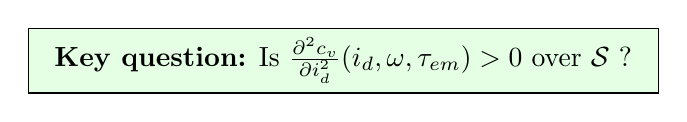
\begin{tikzpicture}
    \node[draw,rectangle,fill=green!10,minimum width=8cm,minimum height=0.8cm]{
    \begin{minipage}{7.5cm}\centering
    \textbf{Key question:} Is $\frac{\partial^2 c_v}{\partial i_d^2}(i_d, \omega, \tau_{em} ) > 0$ over $\mathcal{S}$ ?
    \end{minipage}};
    \end{tikzpicture}
    \end{center}
%}
\end{frame}


\begin{frame}{Optimal torque control problem}{Convexity analysis: Voltage constraint}
    \vspace{-0.2cm}
    \textbf{Key question:} Is $\frac{\partial^2 c_v}{\partial i_d^2}(i_d, \omega, \tau_{em} ) > 0$ over $\mathcal{S}$ ?

    %\pause
    \vspace{0.2cm}
    \textbf{Approach:} Multiply by a positive term to simplify
    \begin{equation*}
        h(i_d, \omega, \tau_{em}) = \underbrace{(K_1+K_2 i_d)^4}_{>0} \cdot \frac{\partial^2 c_v}{\partial i_d^2}(i_d, \omega, \tau_{em} )
    \end{equation*}

    \pause
    \vspace{0.1cm}
    This gives a polynomial:
    \begin{equation*}
        h(i_d, \omega, \tau_{em}) = a_4 i_d^4 + a_3 i_d^3 + a_2 i_d^2 + a_1 i_d + a_0
    \end{equation*}
    where $a_i = a_i(\omega,\tau_{em})$

    \pause
    \vspace{0.2cm}
    \begin{center}
    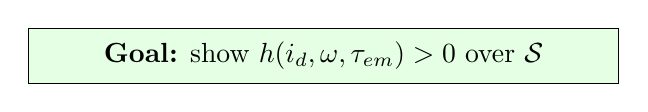
\begin{tikzpicture}
    \node[draw,rectangle,fill=green!10,minimum width=7.5cm,minimum height=0.7cm]{
    \begin{minipage}{7cm}\centering
    \textbf{Goal:} show $h(i_d,\omega,\tau_{em}) > 0$ over $\mathcal{S}$
    \end{minipage}};
    \end{tikzpicture}
    \end{center}
\end{frame}

\begin{frame}{Optimal torque control problem}{Sum-of-Squares (SOS) decomposition}
    \vspace{-0.2cm}
    \textbf{Recall the goal:}
    \begin{center}
    \vspace{-0.1cm}
    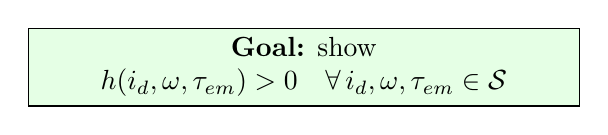
\begin{tikzpicture}
    \node[draw,rectangle,fill=green!10,minimum width=7cm,minimum height=0.7cm]{
    \begin{minipage}{5.5cm}\centering
    \textbf{Goal:} show $h(i_d,\omega,\tau_{em})> 0 \quad \forall \, i_d, \omega, \tau_{em} \in \mathcal{S}$
    \end{minipage}};
    \end{tikzpicture}
    \vspace{-0.1cm}
    \end{center}

    \pause
    \textbf{Proposed approach:} Show that $h$ admits a \textcolor{blue}{\textbf{SoS decomposition}} over $\mathcal{S}$:
    \vspace{-0.1cm}
    \begin{equation*}
        h(i_d,\omega,\tau_{em}) = \textcolor{blue}{s_0} + \textcolor{blue}{s_1}\underbrace{(i_d+i_{max})}_{\geq 0} + \textcolor{blue}{s_2}\underbrace{(-i_d)}_{\geq 0} + \textcolor{blue}{s_3}\underbrace{\omega}_{\geq 0} + \textcolor{blue}{s_4}\underbrace{\tau_{em}}_{\geq 0} \quad \textcolor{blue}{\textbf{(Positivstellensatz)}}
    \end{equation*} 
    \vspace{-0.1cm}
    where each $\textcolor{blue}{s_j}$ is a \textcolor{blue}{\textbf{SoS polynomial}}

    \pause
    \vspace{0.1cm}
    \textbf{What is Sum-of-Squares (SOS)?}
    \vspace{0.1cm}
    \begin{itemize}
        \setlength{\itemsep}{2pt}
        \item Each $\textcolor{blue}{s_j}$ is a \textcolor{blue}{\textbf{sum of squares}}: $s_j = \sum_{k} p_{j,k}^2 \geqslant 0$. \textit{Ex:} $s_0 = (i_d + \omega)^2 + (2\tau_{em} - 1)^2$
        \pause
        %\item Over $\mathcal{S}$, multipliers $(i_d+i_{max})$, $(-i_d)$, $\omega$, $\tau$ are $\geq 0$
        %\pause
        %\item Thus: $h = s_0 + s_1 (i_d+i_{max}) + \cdots \geq 0$ over $\mathcal{S}$ \textcolor{blue}{\textbf{(Positivstellensatz)}}
       % \pause
        \item SOS found via \textcolor{blue}{\textbf{semidefinite programming}} (YALMIP + MOSEK)
    \end{itemize}
\end{frame}

\begin{frame}{Optimal torque control problem}{Convexity via hybrid analytical-SoS approach}
    \begin{proposition}
    For a given PMSM, the reformulated problem is \textcolor{blue}{\textbf{convex}} if one of the following holds:

    \vspace{0.2cm}
    \textcolor{red}{\textbf{1.}} \textbf{Direct SoS approach:} $h$ admits a SoS decomposition
    \begin{equation*}
        h(i_d,\omega,\tau_{em}) = s_0 + s_1(i_d+i_{max}) + s_2(-i_d) + s_3\omega + s_4\tau_{em}
    \end{equation*}
    where each $s_j$ is a \textcolor{blue}{\textbf{SoS polynomial}}.

    \only<1>{
    \vspace{0.2cm}
    \textcolor{gray}{\textcolor{red}{\textbf{2.}} \textbf{Hybrid approach:} $h = h_1 + h_2$ with}
    \begin{equation*}
        \textcolor{gray}{
        \begin{cases}
            h_1(i_d,\omega,\tau_{em}) \geqslant 0 \text{ (proven analytically), } \quad \forall (i_d,\omega, \tau_{em}) \in \mathcal{S}\\
            h_2(i_d,\omega,\tau_{em}) = s_0 + s_1(i_d+i_{max}) + s_2(-i_d) + s_3\omega + s_4\tau_{em}
        \end{cases}
        }
    \end{equation*}
    \textcolor{gray}{where each $s_j$ is a SoS polynomial, ensuring $h \geqslant 0$ over $\mathcal{S}$.}
    }

    \only<2>{
    \vspace{0.2cm}
    \textcolor{red}{\textbf{2.}} \textbf{Hybrid approach:} $h = h_1 + h_2$ with
    \begin{equation*}
        \begin{cases}
            h_1(i_d,\omega,\tau_{em}) \geqslant 0 \text{ (\textcolor{blue}{\textbf{proven analytically}}), } \quad \forall (i_d,\omega, \tau_{em}) \in \mathcal{S}\\
            h_2(i_d,\omega,\tau_{em}) = s_0 + s_1(i_d+i_{max}) + s_2(-i_d) + s_3\omega + s_4\tau_{em}
        \end{cases}
    \end{equation*}
    where each $s_j$ is a \textcolor{blue}{\textbf{SoS polynomial}}, ensuring $h \geqslant 0$ over $\mathcal{S}$.
    }

    \vspace{0.2cm}
    {\small where $h(i_d, \omega, \tau_{em}) = (K_1+K_2 i_d)^4 \cdot c_v''(i_d, \omega, \tau_{em})$ and $\mathcal{S} = \{(i_d, \omega, \tau_{em}) \in \mathbb{R}^3 \:|\: -i_{max} \leqslant i_d \leqslant 0, \: \omega \geqslant 0, \: \tau_{em} \geqslant 0\}$.}
    \end{proposition}
\end{frame}

% \subsection{Direct SoS approach}
% \begin{frame}{Optimal torque control problem}{Proof sketch: Direct SoS approach}
%     %\begin{proof}
%     If $h$ admits the SoS decomposition
%     \begin{equation*}
%         h(i_d,\omega,\tau) = s_0 + s_1(i_d+i_{max}) + s_2(-i_d) + s_3\omega + s_4\tau
%     \end{equation*}
%     where each $s_j$ is a \textcolor{green}{\textbf{SoS polynomial}}, then:

%     \pause
%     \vspace{0.2cm}
%     \textbf{Step 1:} Each $s_j$ is a sum of squares, so
%     \begin{equation*}
%         s_j(i_d,\omega,\tau) = \sum_{k} p_{j,k}^2(i_d,\omega,\tau) \geqslant 0, \quad \forall (i_d,\omega,\tau) \in \mathbb{R}^3
%     \end{equation*}
%     \textit{Example:} $s_0(i_d,\omega,\tau) = (i_d + \omega)^2 + (2\tau - 1)^2 + \omega^2$ is a SoS polynomial

%     \pause
%     \vspace{0.2cm}
%     \textbf{Step 2:} Over the domain $\mathcal{S} = \{(i_d, \omega, \tau) \in \mathbb{R}^3 \:|\: -i_{max} \leqslant i_d \leqslant 0, \: \omega \geqslant 0, \: \tau \geqslant 0\}$, the multipliers are non-negative:
%     \begin{equation*}
%         \underbrace{(i_d+i_{max})}_{\geqslant 0}, \quad \underbrace{(-i_d)}_{\geqslant 0}, \quad \underbrace{\omega}_{\geqslant 0}, \quad \underbrace{\tau}_{\geqslant 0}
%     \end{equation*}

%     \pause
%     \vspace{0.2cm}
%     \textbf{Step 3:} Therefore, $h(i_d,\omega,\tau) \geqslant 0$ over $\mathcal{S}$ (\textcolor{blue}{\textbf{Positivstellensatz certificate}}).

%     \pause
%     \vspace{0.2cm}
%     This certificate can be \textcolor{green}{\textbf{found computationally}} using semidefinite programming (YALMIP + MOSEK).
%    % \end{proof}
% \end{frame}

% \begin{frame}{Optimal torque control problem}{Drawbacks of direct SOS approach}
%         \textbf{Challenge:} Direct SoS decomposition of the entire polynomial may be:
%     \begin{itemize}
%         \item Computationally expensive (high degree, many variables)
%         \item Numerically difficult to find
%         \item May not exist for a fixed degree of polynomial $s_j$ even when $h \geqslant 0$ is true
%     \end{itemize}
% \end{frame}
% \subsection{Proof sketch}
% \begin{frame}{Optimal torque control problem}{Proof sketch: Hybrid analytical-SOS approach}
%     \textbf{Goal:} Prove that a polynomial $h(i_d, \omega, \tau) \geqslant 0$ over domain $\mathcal{S}$.

%     \pause
%     \vspace{0.3cm}
%     \textcolor{blue}{\textbf{Key idea:}} Decompose $h = h_1 + h_2$ where:
%     \begin{center}
%     \begin{tabular}{cc}
%         \tikz[baseline]{\node[rectangle, draw=green!60!black, thick, fill=green!10, inner sep=5pt, align=center] (analytical) {
%             \textbf{Analytical proof} \\[0.2cm]
%             Part of polynomial \\
%             where signs are \\
%             easy to determine
%         };}
%         &
%         \tikz[baseline]{\node[rectangle, draw=orange!60!black, thick, fill=red!10, inner sep=5pt, align=center] (sos) {
%             \textbf{SoS proof} \\[0.2cm]
%             Remaining part \\
%             where SoS \\
%             is more tractable
%         };}
%     \end{tabular}

%     \end{center}

% \end{frame}

\subsection{Practical example}
\begin{frame}{Optimal torque control problem}{A practical example PMSM}
    \vspace{-0.3cm}
    Consider the PMSM test bench available in the Ampère Laboratory:
\begin{columns}
    \begin{column}{0.5\framewidth}
        \begin{table}[!h]
            \small
            %\caption{PMSM parameters.}
            \centering
            \begin{tabular}{cc}
            \toprule
            \textbf{Parameter} & \textbf{PMSM}\\
                \midrule
                Resistance $R$ $(\Omega)$        & 0.9\\
                $d$-axis inductance $L_d$ $(mH)$   & 0.012\\
                $q$-axis inductance $L_q$ $(mH)$   & 0.020\\
                Flux constant $\phi_f$ $(mWb)$  	 & 0.264\\
                Pole pairs $p$       			 & 4     \\
                DC voltage $v_{\mathrm{DC}}$ $(V)$ & 600 \\
                Maximum power $P$ $(kW)$		     & 15\\
                \bottomrule
            \end{tabular}
            \label{tab:IPMSM_parameters}
        \end{table}
    \end{column}
    \begin{column}{0.5\framewidth}
        \begin{figure}[H]
            \centering
            \includegraphics[trim={0cm 5cm 2cm 0cm},clip,width=0.8\textwidth]{pictures/Banc_IPMSM.eps}
            \caption{ PMSM test bench.}
            \label{fig:bancIPMSM}
        \end{figure}
    \end{column}
\end{columns}
    \begin{equation*}
        h(i_d, \omega, \tau_{em}) = \tikz[remember picture,baseline=(h1.base)]{\node[inner sep=2pt](h1){$\textcolor{blue}{\underbrace{a_4(\omega,\tau_{em}) i_d^4 + a_3(\omega,\tau_{em}) i_d^3 + a_2(\omega,\tau_{em}) i_d^2}_{h_1(i_d,\omega, \tau_{em})}}$};} + \tikz[remember picture,baseline=(h2.base)]{\node[inner sep=2pt](h2){$\textcolor{red}{\underbrace{a_1(\omega,\tau_{em}) i_d + a_0(\omega,\tau_{em})}_{h_2(i_d, \omega,\tau_{em} )}}$};}
    \end{equation*}
    \vspace{-0.1cm}
    \begin{itemize}
        \item $h_1(i_d,\omega,\tau_{em}) > 0 \quad \forall\, i_d,\,\omega,\, \tau_{em} \in \mathcal{S}$ is shown analytically
        \item $h_2(i_d,\omega,\tau_{em}) > 0 \quad \forall\, i_d,\,\omega,\, \tau_{em} \in \mathcal{S}$ is shown through SoS decomposition
    \end{itemize}
\end{frame}

\begin{frame}{Optimal torque control problem}{A practical example PMSM}
\begin{columns}
    \begin{column}{0.5\textwidth}
        The optimal torque control problem
        \begin{eqnarray*}
&\underset{i_d}{\textbf{min}} \quad f(i_d,\tau_{em})\quad \textbf{such that}\\
&c_i(i_d,\tau_{em})\leqslant0\\
&c_v(i_d,\omega,\tau_{em})\leqslant0\\
\end{eqnarray*}
over the domain of definition $\mathcal{S}$ is \textbf{\textcolor{OliveGreen}{convex}}

 \only<2>{
    \vspace{+0.5cm}
We implement:
 \begin{center}
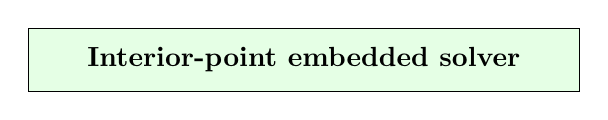
\begin{tikzpicture}
\node[draw,rectangle,fill=green!10,minimum width=7cm,minimum height=0.8cm]{
\begin{minipage}{6.5cm}\begin{center}
\textbf{Interior-point embedded solver}
\end{center}\end{minipage}};
\end{tikzpicture}
\end{center}
 }
    \end{column}
    \begin{column}{0.5\textwidth}
            \begin{figure}[H]
            \centering
            \includegraphics[trim={0cm 5cm 2cm 0cm},clip,width=0.8\textwidth]{pictures/Banc_IPMSM.eps}
            \caption{ PMSM test bench.}
            \label{fig:bancIPMSM}
        \end{figure}
    \end{column}
\end{columns}

\end{frame}
\begin{frame}{Optimal torque control problem}{Experiment results}


    \begin{columns}
        \begin{column}{0.5\textwidth}
            \begin{figure}[h!]
            \centering
                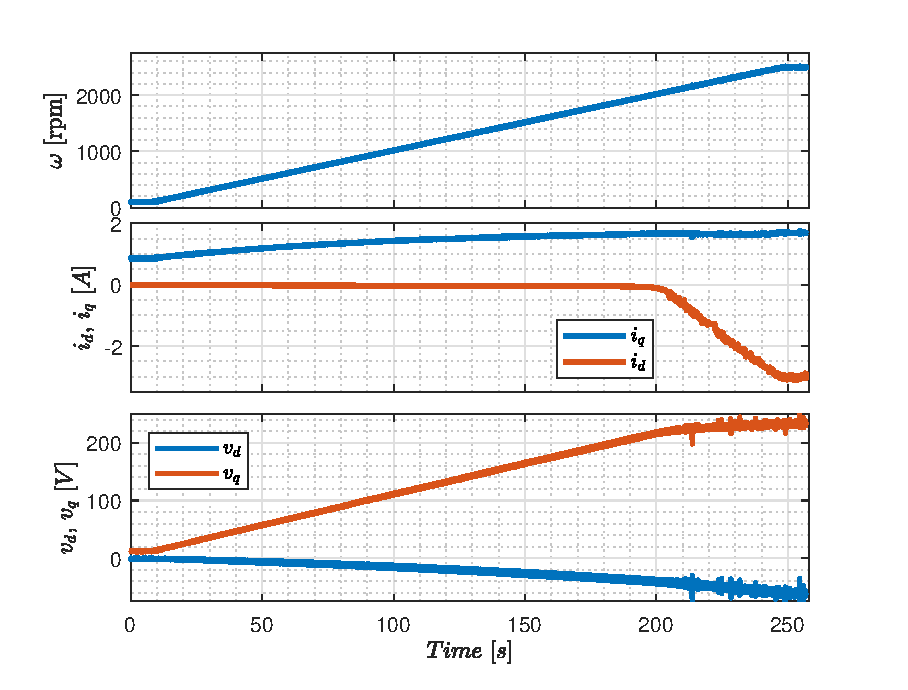
\includegraphics[width=1\columnwidth]{pictures/speed_idq_vdq1.eps}
            \end{figure}
        \end{column}
        \begin{column}{0.5\textwidth}
             \begin{figure}[h!]
            \centering
                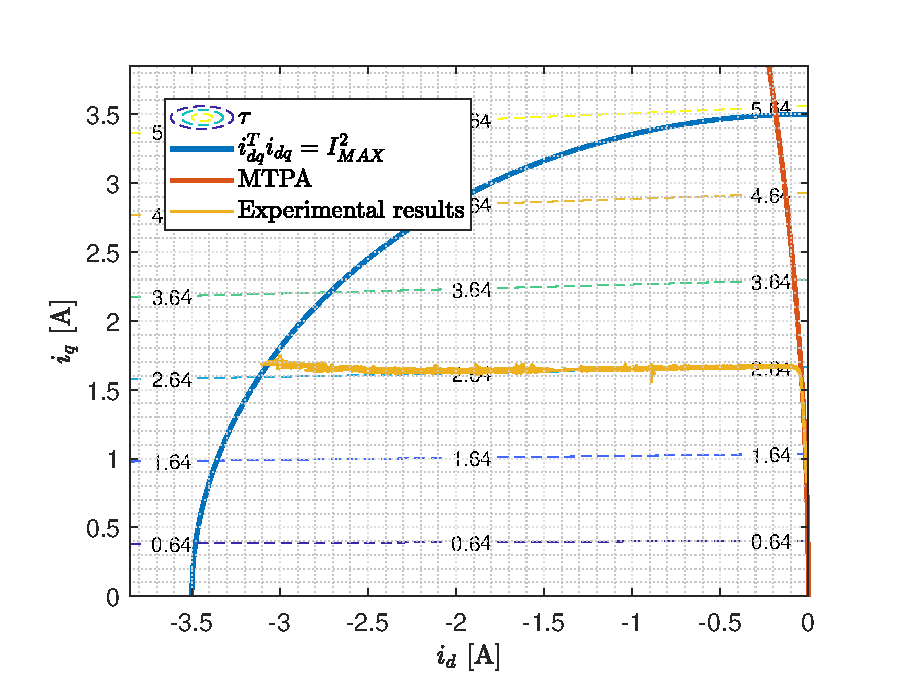
\includegraphics[width=1\columnwidth]{pictures/expe_idq_solver.eps}
            \end{figure}
        \end{column}
    \end{columns}

%     \vspace{-0.3cm} \begin{figure}[h!]
%     \centering
%     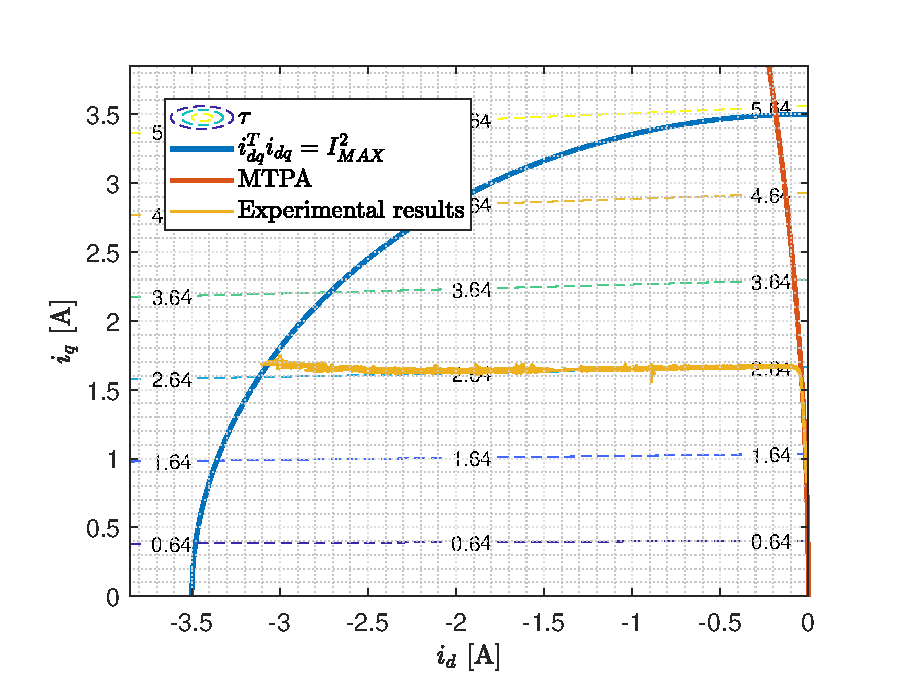
\includegraphics[width=0.7\textwidth]{pictures/expe_idq_solver.eps}
%     %\caption{Currents $i_{dq}$ trajectory in the $dq$ frame}
%     \label{fig:Experimental_Validation_Idq}
% \end{figure}
\end{frame}

\begin{frame}{Result Summary}
    \textbf{Challenge:} A nonconvex Optimal torque control problem
    \vspace{+0.2cm}
    %\textbf{Optimal Torque Control: Key achievements}

    \vspace{0.2cm}
    \begin{columns}
        \begin{column}{0.5\textwidth}
            \textbf{Theoretical contributions:}
            \begin{itemize}
                \item Change of variable
                \item New formulation of OTC problem
                \item Proof of Convexity via Sum-of-Squares programming
            \end{itemize}

            \vspace{0.1cm}
            \textbf{Implementation:}
            \begin{itemize}
                \item Interior-point embedded solver
            \end{itemize}
        \end{column}

        \begin{column}{0.5\textwidth}
            \textbf{Advantages:}
            \begin{itemize}
                \item[$+$] Polynomial complexity solvers
                \item[$+$] Scales well
                \item[$+$] Easy integration into larger convex problems
                \item[$+$] Unified solution for all operating regions
                \item[$+$] Experimental validation on PMSM test bench
            \end{itemize}
        \end{column}
    \end{columns}

    % \vspace{0.3cm}C
    % \centering
    % \textcolor{OliveGreen}{\textbf{$\Rightarrow$ Guaranteed convex optimization for optimal torque control}}
\end{frame}

\begin{frame}{Outline}
        % The outline
                \textbf{Objectives:}
    \vspace{0.2cm}
    \begin{enumerate}
        \item[\textcolor{darkgray}{\textbf{Part 1:}}] \textcolor{darkgray}{\textbf{Optimal currents $i_d^\#$, $i_q^\#$ to produce desired torque $\tau_{em}$ and speed $\omega$ ?}}
        \item[\textcolor{Magenta4}{\textbf{Part 2:}}] \textcolor{Magenta4}{\textbf{Embedded closed-loop control synthesis}}
        \item[\textcolor{darkgray}{\textbf{Part 3:}}] \textcolor{darkgray}{\textbf{New control approaches}}
    \end{enumerate}
        \begin{figure}
            \begin{center}
                \def\textsize{.8}
                \psfrag{Algo}[c][c][1]{\color{Blue4}Control}
                \psfrag{Control}[c][c][1]{\color{gray}Control}
                \psfrag{iabc}[c][c][\textsize]{\color{Blue4}$i_{abc}$}
                \psfrag{idq}[c][c][\textsize]{\color{Blue4}$i_{dq}$}
                \psfrag{vabcr}[c][c][\textsize]{\color{Blue4}$v_{abc}^\#$}
                \psfrag{vdqr}[c][c][\textsize]{\color{Blue4}$v_{dq}^\#$}
                \psfrag{dq}[c][c][.5]{\color{Blue4}${dq}$}
                \psfrag{abc}[c][c][.5]{\color{Blue4}${abc}\quad$}
                \psfrag{S}[c][c][\textsize]{\color{Blue4}$S_{abc}$}
                \psfrag{MLI}[c][c][\textsize]{\color{Blue4}Mod}
                \psfrag{ParkInv}[c][c][.5]{}
                \psfrag{Park}[c][c][.5]{}
                \psfrag{TS1}[l][c][.6]{\color{Blue4}Higher priority $\approx20$kHz}
                % Reference generation (cyan) - lower priority optimization
                \psfrag{Vr}[c][c][\textsize]{\color{Cyan4}$\rho^\#$}
                \psfrag{ref}[c][c][\textsize]{\color{gray}$\omega^\#$}
                \psfrag{ref2}[c][c][\textsize]{\color{gray}$i_d^\#$}
                \psfrag{ref3}[c][c][\textsize]{\color{gray}$\omega^\#$}
                \psfrag{ref4}[c][c][\textsize]{\color{gray}$i_q$}
                \psfrag{ref5}[c][c][\textsize]{\color{Magenta4} Specification}
                \psfrag{ref6}[c][c][\textsize]{\color{Magenta4} Model}
                \psfrag{Reference}[c][c][\textsize]{\color{gray}Trajectory}
                \psfrag{calculation}[c][c][\textsize]{\color{gray}generation}
                \psfrag{TS2}[l][c][.6]{\color{Cyan4}Lower priority $\approx1$kHz}
                % Embedded synthesis (magenta) - idle task
                \psfrag{Emb}[c][c][\textsize]{\color{Magenta4}Embedded}
                \psfrag{Synt}[c][c][\textsize]{\color{Magenta4}synthesis}
                \psfrag{K}[c][c][\textsize]{\color{Magenta4}K}
                \psfrag{TS3}[l][c][.6]{\color{Magenta4}Idle task}
                % Physical system (red) - PMSM and measurements
                \psfrag{Onduleur}[c][c][\textsize]{\color{Red4}Inverter}
                \psfrag{PMSM}[c][c][\textsize]{\color{Red4}PMSM}
                \psfrag{V}[c][c][\textsize]{\color{Red4}$v_{abc}$}
                \psfrag{th}[c][c][\textsize]{\color{Red4}$\theta$}
                \psfrag{w}[c][c][\textsize]{\color{Red4}$\omega$}
                \psfrag{thm}[c][c][\textsize]{\color{Red4}$\theta$}
                \psfrag{wm}[c][c][\textsize]{\color{Red4}$\omega$}
                \psfrag{Embedded}[l][c][.7]{\color{red}Embedded code}
                \includegraphics[width = .9\textwidth]{pictures/AdvancedControl_embbeded1.eps}
            \end{center}
        \label{fig:AdvencedControlForElectricalMotor}
        \end{figure}
\end{frame}
